\subsubsection{The Issue of Candidate Multiplicity}
\label{subsec:issue-of-candidate-multiplicity}
The background sample is dominated by candidates that come from events with a high candidate-multiplicity at the level of baseline selection as seen in figure~\ref{fig:candidate-multiplicity}.
\begin{figure}[!ht]
\centering
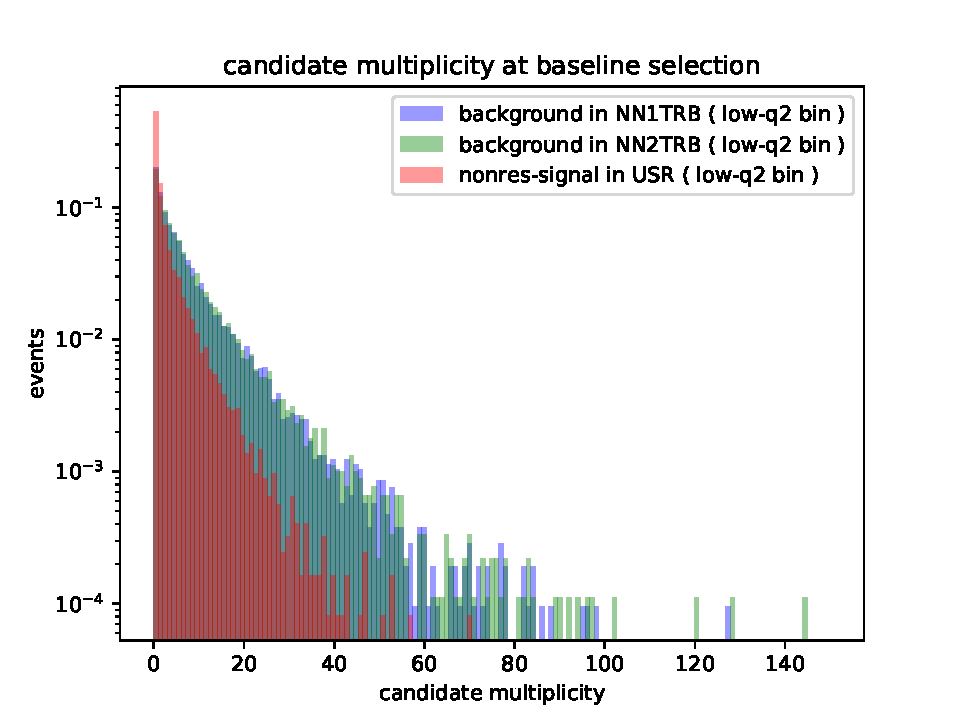
\includegraphics[width=0.6\textwidth]{figures/candidate-multiplicity-by-events.pdf}
\caption{Normalized candidate multiplicities for the non--truth matched \BeeKStar MC signal sample in the USR (red), the data in side--bands of \mB (SB1-\mB and SB2-\mB, in blue) and the data in the same-sign charge side--band (SBQ-SS$_{\rm tt}$, in green). All three distributions are given in the \lowqs bin. For this illustration, the two data distributions include only a small fraction of the full data-set.}
\label{fig:candidate-multiplicity}
\end{figure}
The high candidate-multiplicity is largely due to the corresponding high multiplicity of ID tracks (and possibly also electrons).

Thus, an NN model trained on such a background sample is preoccupied with learning to reject a small number of events with a high value of candidate-multiplicity.
This would lead to an apparently acceptable background rejection at the level of candidates but poor performance in terms of the rejection rate for background events.
Thus, we need to find a procedure that will allow us to narrow down the list of candidates (per event) that is used for the NN training.

Handling multiplicity is not a major issue for the signal per se as we can train the NN models on MC signal samples made of truth-matched candidates only.
Thus, it should be noted that candidate-multiplicity at the level of baseline selection is purely an issue for the background training sample.

Once we have a strategy to get a sample on which we can train the NN, the selection of a single candidate per event after the application of the NN is to be done purely based on the NN scores (i.e. starting from the full list of candidates, regardless of the multiplicity).
This final decision can be done in several ways, based on some predefined prescription depending on the two NN scores, etc.

A strategy to reduce the candidate-multiplicity should be such that it retains such candidate that are most ``signal-like'' in any event.
This is to ensure that when we reduce the number of candidates in large multiplicity events, we are not only keeping such candidates that the NN can differentiate from the signal rather trivially.
Since the purpose of this choice is to not be a strict one, but rather to simply ensure that the training of the NN is not unreasonably biased, we choose a loose level of candidate-multiplicity reduction, based on the best $N\sim 5$ candidates according to one of the available features that characterise the decay.
This also allows adequate statistics for the background training sample, particularly when it is split across several regions, training/testing, etc.

We analyze three different classes of strategies for the reduction of candidate multiplicity: selecting the \emph{best-N} candidates per each event where ``best'' is defined as having the lowest $\chi^2_{B}$, the highest $L_{\rm xy}^\text{sig}$, and the highest $L_{\rm xy}^\text{sig}/\chi^2(B))$, respectively, where $L_{\rm xy}^\text{sig}$ is the transverse decay length  significance (the value itself divided by its error) and where $\chi^2_{B}$ is the four-track vertex goodness of fit parameter.
The quantity $L_{\rm xy}^\text{sig}/\chi^2(B))$ is physically well--motivated since it is simultaneously preferring ``good and significantly displaced'' decays, as expected from the signal.
While the $\chi^2_{B}$ alone is also motivated, it is less so compare to the ratio, since there could be many background candidates having a good vertex fit but without any displacement.

The ``$N$'' in the ``best $N$'' refers to the number of candidates that we retain per each event for the training.
A proxy measure of how effectively a strategy retains the ``signal-like'' candidates of an event is straightforwardly quantitative, we simply calculate the efficiency with which a given strategy retains the truth--matched candidate of an event in the MC sample of non-resonant signal in USR (\lowqs bin).
These truth--efficiencies for the strategies listed above are tabulated in table \ref{tab:truth-efficiencies-baseline-selection}.
\begin{table}[!ht]
\centering
\caption{Truth--efficiency of candidate--multiplicity, $N$, reduction strategies computed using the \BeeKStar signal sample. If we set the threshold at efficiency $>99\%$, the $L_{\rm xy}^\text{sig}/\chi^2_{B}$ and $L_{\rm xy}^\text{sig}$ give consistent results for $N\geq 6$, while the $\chi^2_{B}$ is worse.}
\label{tab:truth-efficiencies-baseline-selection} 
\vspace{0.1cm}
\begin{tabular}{|| c || c | c | c ||} 
 \hline
$N$ & $L_{\rm xy}^\text{sig}/\chi^2_{B}$ & $L_{\rm xy}^\text{sig}$ & $\chi^2_{B}$ \\
\hline
\hline
1 & 89.4\% & 91.3\% & 83.4\% \\
\hline
2 & 95.6\% & 96.1\% & 91.1\% \\
\hline
3 & 97.3\% & 97.6\% & 94.1\% \\
\hline
4 & 98.3\% & 98.4\% & 95.9\% \\
\hline
5 & 98.8\% & 98.9\% & 97.0\% \\
\hline
6 & 99.1\% & 99.2\% & 97.7\% \\
\hline
7 & 99.3\% & 99.3\%  & 98.2\% \\
\hline
8 & 99.4\% & 99.5\% & 98.6\% \\
\hline
9 & 99.6\% & 99.6\%  & 98.9\% \\
\hline
10 & 99.7\% & 99.7\% & 99.1\% \\
\hline
20 & 99.9\% & 99.9\%  & 99.9\% \\
\hline
30 & 100\% & 100\% & 100\% \\
\hline
% {All Inclusive} & 100\% & 100\% \\
% \hline
\end{tabular}
\end{table}

At a given level of candidate-multiplicity reduction, among different strategies, the more distinctive the background shape is from the signal, the better. This would allow for a more efficient training of the NN. 
Expectedly, as we loosen the choice of the candidate-multiplicity allowed for the training (i.e. increasing $N$), the background shape becomes more and more distinctive from that of the signal.
However, choosing a low level of candidate-multiplicity reduction in order to ``take advantage'' of this behavior would defy the whole purpose of doing the multiplicity analysis in the first place.
That is, the ease of distinction between the background and the signal is coming from such candidates that belong to events with a high candidate multiplicity.
As a result, the NN would only learn to identify such background candidates that are easy to distinguish and are coming from a small number of events.
In other words, it would fail to learn to distinguish between signal and background for the background candidates coming from a large number of events with low candidate-multiplicity.

We currently choose ``best $N=6$ $L_{xy}^{\rm sig}/\chi^2_{B}$'' candidates per event which gives a truth-efficiency of $>99\%$ as can be seen in table~\ref{tab:truth-efficiencies-baseline-selection}.
